\chapter{CORDIC}

The CORDIC algorithm is an iterative method used to compute trigonometric functions such as sine and cosine, as well as other elementary functions, using only shift and add operations. Due to its low hardware complexity, CORDIC is particularly well suited for digital hardware implementations, including FPGA-based designs.

In this report, the internal mathematical details of the CORDIC algorithm are not discussed in depth. For an intuitive explanation and a visual overview of the underlying principles, the reader is referred to \href{https://www.youtube.com/watch?v=bre7MVlxq7o}{this video} by Bobater on YouTube.

Within this project, the CORDIC functionality is implemented through two main modules. The first module corresponds to the core CORDIC unit, which performs the iterative angle computation. The second module acts as a wrapper, and is responsible for handling sign corrections and quadrant mapping in order to extend the computation to the full trigonometric domain.

In the current implementation, the CORDIC module operates as a standalone component and is not directly integrated into the CPU datapath. The module can be controlled and tested independently from the processor core. However, due to the modular structure of the overall design, the CORDIC unit can be integrated as part of the CPU in future extensions, for example as a dedicated functional unit or coprocessor.

\pagebreak
\section{CORDIC Core}

\begin{figure}[H]
  \centering
  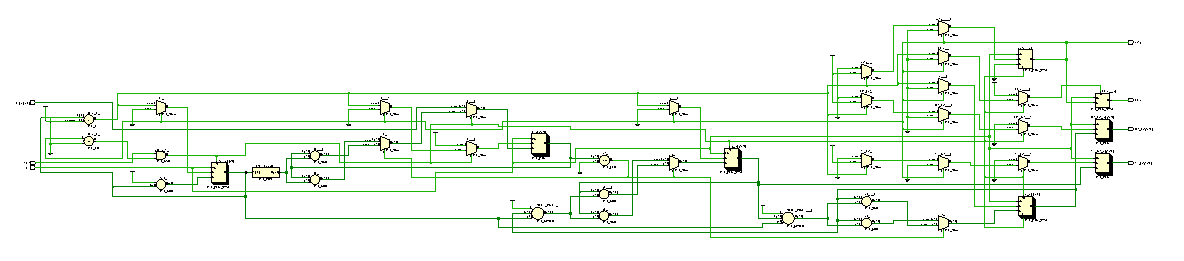
\includegraphics[width=\textwidth]{images/cordic.pdf}
  \caption{High-level overview of the CORDIC core as rendered by Vivado.}
  \label{fig:cordic_core}
\end{figure}

The CORDIC core implements the core computational engine used to evaluate trigonometric functions. Given an input angle within the range $[-\pi/2, +\pi/2]$, the module computes the corresponding sine and cosine values using an iterative shift-and-add algorithm. This approach is well suited for hardware implementations, as it avoids the use of multipliers and relies only on additions, subtractions, and arithmetic shifts.

The module operates in rotation mode and uses fixed-point arithmetic to represent both the input angle and the output values. The input angle is represented using a signed fixed-point format, while the sine and cosine outputs are provided in a normalized fixed-point representation. The number of iterations and the numerical precision are configurable through generic parameters, allowing a trade-off between accuracy and latency.

The interface of the CORDIC core is reported in Listing~\ref{lst:cordic_core}. The entity exposes the control signals required to start the computation, the input angle, and the output signals carrying the computed sine and cosine values, together with status flags indicating the progress and completion of the operation.

{\scriptsize
\begin{lstlisting}[
    caption={Entity declaration of the CORDIC core.},
    label={lst:cordic_core},
    breaklines=true,
    breakatwhitespace=true,
    columns=flexible
]
entity cordic_core is
    generic (
        WIDTH      : integer := 16;
        ITERATIONS : integer := 16
    );
    port (
        clk     : in  std_logic;
        start   : in  std_logic;
        angle   : in  signed(WIDTH-1 downto 0); -- Q2.(WIDTH-2)

        busy    : out std_logic;
        done    : out std_logic;

        cos_out : out signed(WIDTH-1 downto 0); -- Q1.(WIDTH-1)
        sin_out : out signed(WIDTH-1 downto 0)  -- Q1.(WIDTH-1)
    );
end cordic_core;
\end{lstlisting}
}

Internally, the core maintains three state variables representing the current vector components and the residual angle. At each iteration, the algorithm updates these values according to the sign of the residual angle, progressively rotating the vector towards the target angle. A constant scaling factor is applied to compensate for the intrinsic gain introduced by the CORDIC iterations. The arctangent values required by the algorithm are stored in a precomputed lookup table.

The computation is initiated by asserting a start signal. While the computation is in progress, the core signals a busy condition. Once all iterations have been completed, the resulting sine and cosine values are produced at the outputs and a done signal is asserted for one clock cycle. This handshake-based interface simplifies the integration of the CORDIC core within larger systems, such as the wrapper and the board-level top module.

The correct functionality of the CORDIC core has been verified through a dedicated testbench. In order to improve the readability of the results, the fixed-point sine and cosine outputs are converted to decimal values during simulation.

Figure~\ref{fig:tb_cordic_core} shows the simulation results obtained for a set of representative input angles, namely 15°, 30°, 45°, and 60°.

\begin{figure}[H]
  \centering
  \includegraphics[width=\textwidth]{images/tb_cordic_core.png}
  \caption{Simulation results of the CORDIC core testbench as rendered by Vivado.}
  \label{fig:tb_cordic_core}
\end{figure}

The obtained results match the expected values with good accuracy. However, a limitation of the current implementation must be highlighted. The CORDIC algorithm exhibits incorrect sign behavior for specific edge cases, in particular for angles equal to zero or exact multiples of $\pi/2$. While the computed magnitude of sine and cosine is correct, the sign of one or both outputs may be incorrect in these boundary conditions.

This behavior is related to the iterative nature of the CORDIC rotation mode. Even for angles that theoretically require no rotation (such as zero), the algorithm still performs a sequence of micro-rotations. Due to finite precision and the sign-based update rule, these iterations can converge to a value with the correct magnitude but an incorrect sign in specific corner cases.

A possible workaround would consist in explicitly detecting these critical angles and overriding the output values with predefined results. However, such an approach would partially compromise the purely iterative nature of the CORDIC algorithm and introduce special-case handling logic. For this reason, this limitation is documented but not addressed in the current implementation.

\pagebreak
\section{CORDIC Wrapper}

\begin{figure}[H]
  \centering
  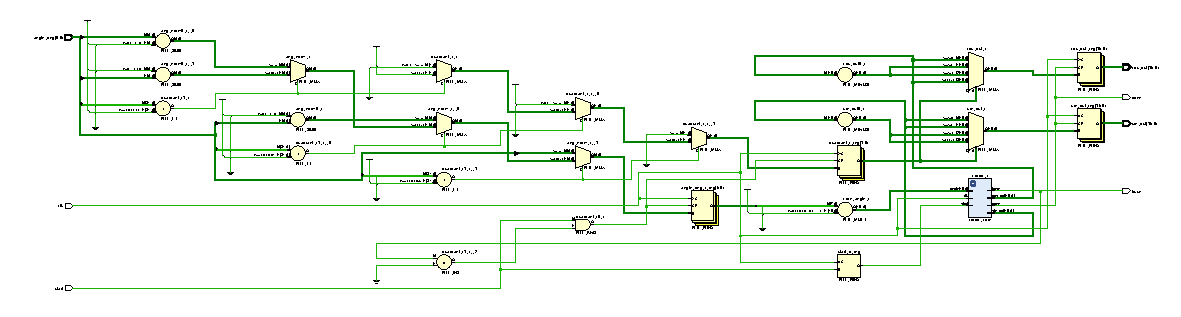
\includegraphics[width=\textwidth]{images/cordic_wrapper.pdf}
  \caption{High-level overview of the CORDIC wrapper as rendered by Vivado.}
  \label{fig:cordic_wrapper}
\end{figure}

The CORDIC wrapper extends the functionality of the CORDIC core in order to support the full trigonometric domain. While the CORDIC core operates correctly only for input angles within the range $[-\pi/2, +\pi/2]$, the wrapper enables the computation of sine and cosine for angles spanning the full circle. This is achieved by mapping the input angle to the corresponding equivalent angle within the valid range of the core and by applying the appropriate sign corrections based on the quadrant of the original angle.

The wrapper therefore performs angle normalization, quadrant identification, and output sign adjustment, while delegating the actual trigonometric computation to the underlying CORDIC core. This approach preserves the modularity of the design and allows the core algorithm to remain unchanged.

The interface of the CORDIC wrapper is reported in Listing~\ref{lst:cordic_wrapper_entity}. The entity receives the input angle expressed in degrees in the range from 0 to 359 and provides the corresponding sine and cosine values in fixed-point format, together with handshake signals indicating the computation status.

{\scriptsize
\begin{lstlisting}[
    caption={Entity declaration of the CORDIC wrapper.},
    label={lst:cordic_wrapper_entity},
    breaklines=true,
    breakatwhitespace=true,
    columns=flexible
]
entity cordic_wrapper is
    generic (
        WIDTH      : integer := 16;
        ITERATIONS : integer := 16
    );
    port (
        clk       : in  std_logic;
        start     : in  std_logic;
        angle_deg : in  unsigned(8 downto 0); -- 0..359

        busy      : out std_logic;
        done      : out std_logic;

        cos_out   : out signed(WIDTH-1 downto 0);
        sin_out   : out signed(WIDTH-1 downto 0)
    );
end cordic_wrapper;
\end{lstlisting}
}

The wrapper has been validated through a dedicated testbench in which the sine and cosine outputs are converted to decimal values for ease of interpretation. In order to verify the correct handling of angle mapping and quadrant-dependent sign assignment, the following angles have been tested: 45°, 135°, 225°, and 315°.

\begin{figure}[H]
  \centering
  \includegraphics[width=\textwidth]{images/tb_cordic_wrapper.png}
  \caption{Simulation results of the CORDIC wrapper testbench as rendered by Vivado.}
  \label{fig:tb_cordic_wrapper}
\end{figure}

As expected, the magnitude of the sine and cosine values remains consistent across the tested angles, while the signs change according to the corresponding quadrant. This behavior confirms the correct implementation of the quadrant mapping and sign correction logic within the wrapper module.
